% !TEX root = ../main.tex

\section{Theory}

\subsection{Notations and definitions}

Matrices of size $N$ rows and $M$ columns are denoted by boldface capital letters, e.g., $\mathbf{X} \in \mathbb{R}^{N\times M}$, whereas column vectors of length $N$ are denoted as boldface lowercase letters, e.g., $\mathbf{x} \in \mathbb{R}^{N}$. Scalars are denoted by lowercase letters, e.g., $k$. Continuous functions are denoted by brackets, e.g., $h(t)$, while discrete functions are denoted by square brackets, e.g., $x[k]$. The Euclidean norm of a matrix $\mathbf{X}$ is denoted as $\|\mathbf{X}\|_2$, the $\ell_1$-norm is denoted by $\| \mathbf{X} \|_1$ and the Frobenius norm is denoted by $\| \mathbf{X} \|_F$. The discrete integration ($\mathbf{L}$) and difference ($\mathbf{D}$) operators are defined as:

$$
\mathbf{L} = \left[\begin{array}{ccccc}
1 & 0 & \ldots & & \\
1 & 1 & 0 & \ldots & \\
1 & 1 & 1 & 0 & \ldots \\
\vdots & \ddots & \ddots & \ddots & \ddots
\end{array}\right], \quad \mathbf{D} = \left[\begin{array}{ccccc}
1 & 0 & \ldots & & \\
1 & -1 & 0 & \ldots & \\
0 & \ddots & \ddots & \ddots & \ldots \\
\vdots & \ddots & 0 & 1 & -1
\end{array}\right].
$$

\subsection{Conventional general linear model analysis}

Conventional general linear model (GLM) analysis puts forward a number of regressors incorporating the knowledge about the paradigm or behavior. For instance, the timing of epochs for a certain condition can be modeled as an indicator function $p(t)$ (e.g., Dirac functions for event-related designs or box-car functions for block-designs) convolved with the hemodynamic response function (HRF) $h(t)$, and sampled at TR resolution (\citealt{Friston1994AnalysisfunctionalMRI,Friston1998EventRelatedfMRI,Boynton1996LinearSystemsAnalysis,Cohen1997ParametricAnalysisfMRI}):
$$
   x(t) = p*h(t) \rightarrow x[k] = p*h(k\cdot\text{TR}).
$$
The vector $\mathbf{x}=[x[k]]_{k=1,\ldots,N}  \in \mathbb{R}^{N}$ then constitutes the regressor modelling the hypothetical response, and several of them can be stacked as columns of the design matrix $\mathbf{X}=[\mathbf{x}_1 \ldots \mathbf{x}_L] \in \mathbb{R}^{N \times L}$, leading to the well-known GLM formulation: 
\begin{equation}
    \label{eq:glm}
    \mathbf{y} = \mathbf{X} \boldsymbol\beta + \mathbf{e},
\end{equation}
where the empirical timecourse $\mathbf{y} \in \mathbb{R}^{N}$ is explained by a linear combination of the regressors in $\mathbf{X}$ weighted by the parameters in $\boldsymbol\beta \in \mathbb{R}^{L}$ and corrupted by additive noise $\mathbf{e}\in \mathbb{R}^{N}$. Under independent and identically distributed Gaussian assumptions of the latter, the maximum likelihood estimate of the parameter weights reverts to the ordinary least-squares estimator; i.e., minimizing the residual sum of squares between the fitted model and measurements. The number of regressors $L$ is typically much less than the number of measurements $N$, and thus the regression problem is over-determined and does not require additional constraints or assumptions (\citealt{HENSON2007178}).

In the deconvolution approach, no prior knowledge of the hypothetical response is taken into account, and the purpose is to estimate the deconvolved activity-inducing signal $\mathbf{s}$ from the measurements $\mathbf{y}$, which can be formulated as the signal model
\begin{equation}
    \label{eq:synthesis_model}
    \mathbf{y} = \mathbf{Hs} + \mathbf{e},
\end{equation}
where $\mathbf{H} \in \mathbb{R}^{N \times N}$ is a Toeplitz matrix that represents the discrete convolution with the HRF, and $\mathbf{s} \in \mathbb{R}^{N}$ is a length-$N$ vector with the unknown activity-inducing signal. Note that the temporal resolution of the activity-inducing signal and the corresponding Toeplitz matrix is generally assumed to be equal to the TR of the acquisition, but it could also be higher if an upsampled estimate is desired. Despite the apparent similarity with the GLM equation, there are two important differences. First, the multiplication with the design matrix of the GLM is an expansion as a weighted linear combination of its columns, while the multiplication with the HRF matrix represents a convolution operator. Second, determining $\mathbf{s}$ is an ill-posed problem given the nature of the HRF. As it can be seen intuitively, the convolution matrix $\mathbf{H}$ is highly collinear (i.e., its columns are highly correlated) due to large overlap between shifted HRFs (see Figure \ref{fig:sim_and_hrf}C), thus introducing uncertainty in the estimates of $\mathbf{s}$ when noise is present. Consequently, additional assumptions under the form of regularization terms (or priors) in the estimate are needed to reduce their variance. In the least squares sense, the optimization problem to solve is given by 
\begin{equation}
    \label{eq:regularized_least_squares}
    \hat{\mathbf{s}} = \arg \min_{\mathbf{s}} \frac{1}{2} \| \mathbf{y} - \mathbf{Hs} \|_2^2 + \Omega(\mathbf{s}).
\end{equation}
The first term quantifies data fitness, which can be justified as the log-likelihood term derived from Gaussian noise assumptions, while the second term \(\Omega(\mathbf{s})\) brings in regularization and can be interpreted as a prior on the activity-inducing signal. For example, the $\ell_2$-norm of $\mathbf{s}$ (i.e., $\Omega(\mathbf{s})=\lambda \left\| \mathbf{s}\right\|_2^2$) is imposed for ridge regression or Wiener deconvolution, which introduces a trade-off between the data fit term and ``energy'' of the estimates that is controlled by the regularization parameter $\lambda$. %Another well-known regularized terms are related to the elastic net (i.e., $\Omega(\mathbf{x})=\lambda_1\|\mathbf{x}\|_2^2 + \lambda_2\|\mathbf{x}\|_1$) [REF]. 
%%%%%%%%%%%%%%%%%%%%%%%%%%%%%%%%%%%%%%%%%%%%%%%%%%%%%%%%%%%%%%%%%%%%%%%%
% Paradigm Free Mapping
%%%%%%%%%%%%%%%%%%%%%%%%%%%%%%%%%%%%%%%%%%%%%%%%%%%%%%%%%%%%%%%%%%%%%%%%

\subsection{Paradigm Free Mapping}
 In paradigm free mapping (PFM), the formulation of Eq.~(\ref{eq:regularized_least_squares}) was considered equivalently as fitting the measurements using the atoms of the HRF dictionary (i.e., columns of $\mathbf{H}$) with corresponding weights (entries of $\mathbf{s}$). This model corresponds to a synthesis formulation. In \citealt{Gaudes2013Paradigmfreemapping} a sparsity-pursuing regularization term was introduced on $\mathbf{s}$, which in a strict way reverts to choosing \(\Omega(\mathbf{s})=\lambda \| \mathbf{s} \|_0\) as the regularization term and solving the optimization problem (\citealt{Bruckstein2009SparseSolutionsSystems}). However, finding the optimal solution to the problem demands an exhaustive search across all possible combinations of the columns of \(\mathbf{H}\). Hence, a  pragmatic solution is to solve the convex-relaxed optimization problem for the \(l_1\)-norm, commonly known as Basis Pursuit Denoising (\citealt{Chen2001BasisPursuitDenoising}) or equivalently as the least absolute shrinkage and selection operator (LASSO) (\citealt{Tibshirani1996RegressionShrinkageSelection}): 
\begin{equation}
    \label{eq:pfm_spike}
    \hat{\mathbf{s}} = \arg \min_{\mathbf{s}} \frac{1}{2} \| \mathbf{y} - \mathbf{Hs} \|_2^2 + \lambda \| \mathbf{s} \|_1,
\end{equation}
which provides fast convergence to a global solution. Imposing sparsity on the activity-inducing signal implies that it is assumed to be well represented by a reduced subset of few non-zero coefficients at the fMRI timescale, which in turn trigger event-related BOLD responses. Hereinafter, we refer to this assumption as the \textit{spike model}. 

%%%%%%%%%%%%%%%%%%%%%%%%%%%%%%%%%%%%%%%%%%%%%%%%%%%%%%%%%%%%%%%%%%%%%%%%
% Total Activation
%%%%%%%%%%%%%%%%%%%%%%%%%%%%%%%%%%%%%%%%%%%%%%%%%%%%%%%%%%%%%%%%%%%%%%%%

\subsection{Total Activation}
Alternatively, deconvolution can be formulated as if the signal to be recovered directly fits the measurements and at the same time satisfies some suitable regularization, which leads to
\begin{equation}
\label{eq:analysis_model}
    \hat{\mathbf{x}} = \arg \min_{\mathbf{x}} \frac{1}{2} \| \mathbf{y} - \mathbf{x} \|_2^2 + \Omega(\mathbf{x}).
\end{equation}
Under this analysis formulation, total variation (TV), i.e., the $\ell_1$-norm of the derivative $\Omega(\mathbf{x})=\lambda \|\mathbf{Dx}\|_1$, is a powerful regularizer since it favors recovery of piecewise-constant signals (\citealt{Chambolle2004TotalVariation}). Going beyond, the approach of generalized TV introduces an additional differential operator $\mathbf{D_H}$ in the regularizer that can be tailored as the inverse operator of a linear system~(\citealt{Karahanoglu2011SignalProcessingApproach}), that is, $\Omega(\mathbf{x})=\lambda \|\mathbf{D D_H x}\|_1$. In the context of hemodynamic deconvolution, Total Activation is proposed for which the discrete operator $\mathbf{D_H}$ is derived from the inverse of the continuous-domain linearized Balloon-Windkessel model (\citealt{Buxton1998BalloonModel,Friston2000Nonlinear-Balloon}). %\todo{I would exclude this part of Equation 6, and refer to the paper of activelets and TA for more information} 
%Exchanging the poles and zeros of the latter's linear-system characterization leads to a differential operator of the form 
%\begin{equation}
%    D_H\ = \prod_{i=1}^{M_1} (D-\alpha_i I) (\prod_{j=1}^{M_2} (D - \gamma_j I))^{-1},
%\end{equation}
%where \(D\) is the derivative operator, \(\alpha_i\) the zeros, and \(\gamma_j\) the poles. 
The interested reader is referred to (\citealt{Khalidov2011ActiveletsWaveletssparse,Karahanoglu2011SignalProcessingApproach,Karahanoglu2013TotalactivationfMRI}) for a detailed description of this derivation. 

Therefore, the solution of the Total Activation (TA) problem
\begin{equation}
\label{eq:TA}
    \hat{\mathbf{x}} = \arg \min_{\mathbf{x}} \frac{1}{2} \| \mathbf{y} - \mathbf{x} \|_2^2 + \lambda \|\mathbf{D D_H x} \|_1
\end{equation}
will yield the activity-related signal $\mathbf{x}$ for which the activity-inducing signal $\mathbf{s}=\mathbf{D_H x}$ and the so-called innovation signal $\mathbf{u}=\mathbf{Ds}$ will also be available, as they are required for the regularization. We refer to modelling the activity-inducing signal based on the innovation signal as the \textit{block model}.

\subsection{Unifying both perspectives}

PFM and TA are based on the synthesis- and analysis-based formulation of the deconvolution problem, respectively. They are also tailored for the spike and block model, respectively. In the first case, the recovered deconvolved signal is synthesized to be matched to the measurements, while in the second case, the recovered signal is directly matched to the measurements but needs to satisfy its analysis in terms of deconvolution. This also corresponds to using the forward or backward model of the hemodynamic system, respectively. Hence, it is possible to make both approaches equivalent (\citealt{Elad2007Analysisversussynthesis})\footnote{Without dwelling into technicalities, for total variation, this equivalence is correct up to the constant, which is in the null space of the derivative operator.}.

To start with, TA can be made equivalent to PFM by adapting it for the spike model; i.e., when removing the derivative operator $\mathbf{D}$ of the regularizer in Eq. (\ref{eq:TA}), it can be readily verified that replacing in that case $\mathbf{x}=\mathbf{Hs}$ leads to identical equations and thus both assume a spike model, since $\mathbf{H}$ and $\mathbf{D_H}$ will cancel out each other (\citealt{Karahanoglu2011SignalProcessingApproach})\footnote{Again, this holds up to elements of the null space.}.

Conversely, PFM spike model can also accommodate the TA block model by modifying Eq. (\ref{eq:pfm_spike}) with the forward model $\mathbf{y} = \mathbf{H L u} + \mathbf{e}$. Here, the activity-inducing signal $\mathbf{s}$ is rewritten in terms of the innovation signal $\mathbf{u}$ as $\mathbf{s}=\mathbf{Lu}$ where the matrix $\mathbf{L}$ is the first-order integration operator (\citealt{Cherkaoui2019SparsitybasedBlind,Urunuela2020StabilityBasedSparse}). This way, PFM can estimate the innovation signal $\mathbf{u}$ as follows: 
\begin{equation}
    \label{eq:pfm_block}
    \hat{\mathbf{u}} = \arg \min_{\mathbf{u}} \frac{1}{2} \| \mathbf{y} - \mathbf{HLu} \|_2^2 + \lambda \| \mathbf{u} \|_1,
\end{equation}
and becomes equivalent to TA by replacing $\mathbf{u}=\mathbf{D D_H x}$, and thus adopting the block model. Based on the previous equations (\ref{eq:pfm_spike}), (\ref{eq:TA}) and (\ref{eq:pfm_block}), it is clear that both PFM and TA can operate under the spike and block models, providing a convenient signal model according to the different assumptions of the underlying neuronal-related signal. This work evaluates the core of the two techniques; i.e., the regularized least-squares problem with temporal regularization without considering the spatial regularization term originally incorporated in TA. For the remainder of this paper, we will use the PFM and TA formalisms with both spike and block models. 

\begin{figure}[t!]
    \begin{center}
        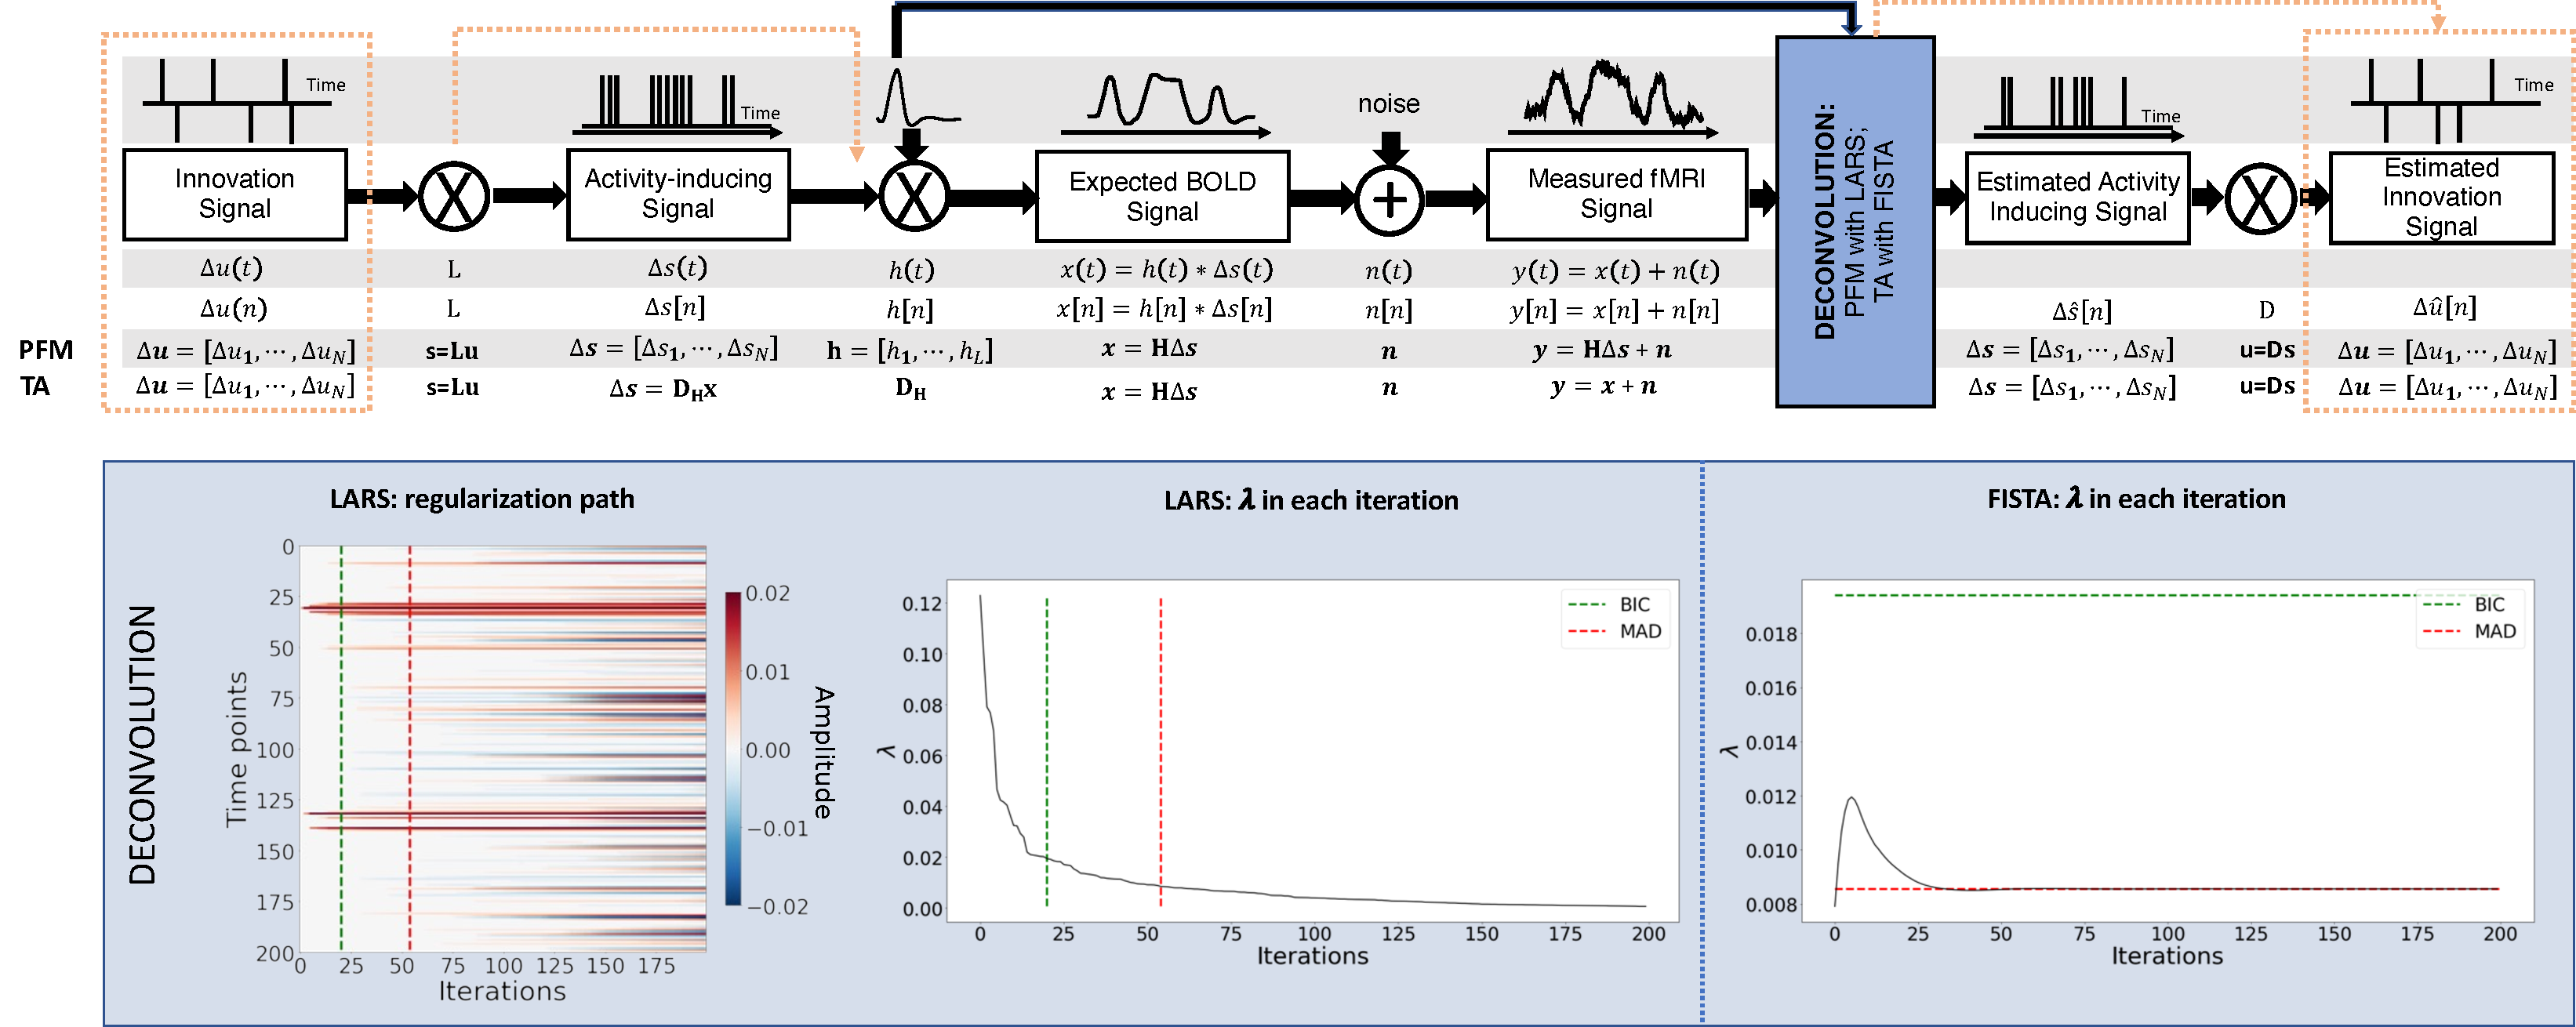
\includegraphics[width=\columnwidth]{figures/flowchart.pdf}
    \end{center}
    \caption{Flowchart detailing the different steps of the fMRI signal and the deconvolution methods described. The orange arrows indicate the flow to estimate the innovation signals. The blue box depicts the iterative \textit{modus operandi} of the two algorithms used in this paper to solve the PFM and TA deconvolution problems. The plot on the left shows the regularization path obtained with LARS, where the x-axis illustrates the different iterations of the algorithm, the y-axis represents points in time, and the color describes the amplitude of the estimated signal. The middle plot depicts the decreasing values of $\lambda$ for each iteration of LARS as the regularization path is computed. The green and r ed dashed lines in both plots illustrate the BIC and MAD solutions, respectively. Comparatively, the changes in $\lambda$ when the FISTA method is made to converge to the MAD estimate of the noise are shown on the right. Likewise, the $\lambda$ corresponding to the BIC and MAD solutions are shown with dashed lines.}
\label{fig:flowchart}
\end{figure}

\subsection{Algorithms and parameter selection}
\label{sec:regparam}
Despite their apparent resemblance, the practical implementations of the PFM and TA methods proposed different algorithms to solve the corresponding optimization problem and select an adequate regularization parameter $\lambda$ (\citealt{Gaudes2013Paradigmfreemapping,Karahanoglu2013TotalactivationfMRI}). The PFM implementation available in AFNI employs the least angle regression (LARS) (\citealt{Efron2004Leastangleregression}), whereas the TA implementation uses the fast iterative shrinkage-thresholding algorithm (FISTA) (\citealt{Beck2009FastIterativeShrinkage}). The blue box in Figure \ref{fig:flowchart} provides a descriptive view of the iterative \textit{modus operandi} of the two algorithms.

On the one hand, LARS is a homotopy approach that computes all the possible solutions to the optimization problem and their corresponding value of $\lambda$; i.e., the regularization path, and the solution according to the Bayesian Information Criterion (BIC) (\citealt{Schwarz1978EstimatingDimensionModel}), was recommended as the most appropriate in the case of PFM approaches since AIC often tends to overfit the signal(\citealt{Gaudes2013Paradigmfreemapping,CaballeroGaudes2019deconvolutionalgorithmmulti}). 

On the other hand, FISTA is an extension of the classical gradient algorithm that provides fast convergence for large-scale problems. In the case of FISTA though, the regularization parameter $\lambda$ must be selected prior to solving the problem, but can be updated in every iteration so that the residuals of the data fit converge to an estimated noise level of the data $\hat{\sigma}$:
\begin{equation}
    \lambda^{n+1} = \frac{N \hat{\sigma}}{\frac{1}{2} \| \mathbf{y} - \mathbf{x}^n \|_F^2} \lambda^n,
\label{eq:std}
\end{equation}
where $x^n$ is the $n^{th}$ iteration estimate, $\lambda^n$ and $\lambda^{n+1}$ are the $n^{th}$ and $n+1^{th}$ iteration values for the regularization parameter $\lambda$, and $N$ is the number of points in the time-course. The pre-estimated noise level can be obtained as the median absolute deviation (MAD) of the fine-scale wavelet coefficients (Daubechies, order 3) of the fMRI timecourse. The MAD criterion has been adopted in TA (\citealt{Karahanoglu2013TotalactivationfMRI}). Of note, similar formulations based on the MAD estimate have also been applied in PFM formulations (\citealt{Gaudes2012Structuredsparsedeconvolution,Gaudes2011MorphologicalPFM}).

% two techniques, i.e., the regularized least-squares problem with temporal regularization, which corresponds to the generalized total-variation operator in Total Activation. Therefore, we do not study the impact of spatial constraints, as we assume that spatial regularization terms should perform identically on both methods.
